% \documentclass[draft,11pt]{article}
\chapter{Different Perspectives on Gaussian
  Elimination}
\label{cha:ge}
% \usepackage{cleveref}
%
%\allowdisplaybreaks

%%% for this lecture
%\newcommand\gap{\text{gap}}
%\newcommand{\Hongjie}[1]{{\color{red} Hongjie: #1}}

%\begin{document}
\sloppy
%\lecture{7 --- Wednesday, April 1}
%{Spring 2020}{Rasmus Kyng}{More Gaussian
  %Elimination,
  %Introduction to Random Matrix Concentration}


\section{An Optimization View of Gaussian Elimination for Laplacians}
In this section, we will explore how to exactly minimize a Laplacian
quadratic form by minimizing over one variable at a time.
It turns out that this is in fact Gaussian Elimination in disguise --
or, more precisely, the variant of Gaussian elimination that we tend
to use on symmetric matrices, which is called Cholesky factorization.

Consider a Laplacian $\LL$ of a connected graph $G = (V,E,\ww)$, where
$\ww \in \R^E$ is a vector of positive edge weights.
Let $\WW \in \R^{E \times E}$ be the diagonal matrix with the edge
weights on the diagonal, i.e. $\WW = \diag(\ww)$ and
$\LL = \BB\WW\BB^\trp$.
Let $\dd \in \R^V$ be a demand vector s.t.\ $ \dd \perp \vecone$.

Let us define an energy
\[
  \energy(\xx) =
-\dd^\trp\xx +
  \frac{1}{2}\xx^\trp\LL\xx
\]
Note that this function is convex and is minimized at $\xx$ s.t.\ $\LL
\xx = \dd$.

We will now explore an approach to solving the minimization problem
\[
\min_{\xx \in \R^V } \energy(\xx)
  \]
%
Let $\xx =
\begin{pmatrix}
  y \\ \zz
\end{pmatrix}$ where $y \in \R$ and $\zz \in \R^{V \setminus
  \setof{1}}$.

We will now explore how to minimize over $y$, given any $\zz$.
Once we find an expression for $y$ in terms of $\zz$,
we will be able to reduce  it to a
new quadratic minimization problem in $\zz$,
\[
  \energy'(\zz) =
-\dd'^\trp\zz +
  \frac{1}{2}\zz^\trp\LL'\zz
\]
where $\dd'$ is a demand vector on the remaining vertices, with $\dd
\perp \vecone$ and $\LL'$ is a Laplacian of a graph on the remaining
vertices $V' = V \setminus \setof{1}$.
We can then repeat the procedure to eliminate another variable and so on.
Eventually, we can then find all the solution to our original
minimization problem.

To help us understand how to minimize over the first variable, we
introduce some notation for the first row and column of the Laplacian:
\begin{equation}
  \label{eq:lapuniformlayout}
  \LL =
\begin{pmatrix}
W & -\aa^\trp \\
-\aa& \diag(\aa) + \LL_{-1}
\end{pmatrix}.
\end{equation}
Note that $W$ is the weighted degree of vertex 1, and that
\begin{equation}
\begin{pmatrix}
W & -\aa^\trp \\
-\aa& \diag(\aa)
\end{pmatrix}
\end{equation}
is the Laplacian of the subgraph of $G$ containing only the edges incident on
vertex 1, while $\LL_{-1}$ is the Laplacian of the subgraph of $G$
containing all edges \emph{not} incident on vertex 1.

Let us also write $\dd =
\begin{pmatrix}
  b \\ \cc
\end{pmatrix}$ where $b \in \R$ and $\cc \in \R^{V \setminus
  \setof{1}}$.

Now,
\begin{align*}
  \energy(\xx)
  &=
  -\dd^\trp\xx +
  \frac{1}{2}\xx^\trp\LL\xx
  =
  -\begin{pmatrix}
  b \\ \cc
\end{pmatrix}^\trp \begin{pmatrix}
  y \\ \zz
\end{pmatrix}
+
  \frac{1}{2}\begin{pmatrix}
  y \\ \zz
\end{pmatrix}^\trp
\left(
\begin{array}{ccc}
W & -\aa^\trp \\
-\aa& \diag(\aa) + \LL_{-1}
\end{array} \right)
\begin{pmatrix}
  y \\ \zz
\end{pmatrix}
  \\
  &=
    - by  -\cc^\trp\zz
    +
    \frac{1}{2}
    \left(
    y^2 W - 2 y \aa^\trp \zz
    +
    \zz^\trp \diag(\aa) \zz
    +
    \zz^\trp \LL_{-1} \zz
    \right).
\end{align*}
Now, to minimize over $y$, we set $\frac{\partial  }{\partial  y}
\energy(\xx) = 0$ and get
\[
    - b
    +
    y W - \aa^\trp \zz
    = 0
   .
  \]
  Solving for $y$, we get that the minimizing $y$ is
\begin{equation}
\label{eq:laponevarmin}
y = \frac{1}{W}(b + \aa^\trp \zz).
\end{equation}

Observe that
\begin{align*}
  \energy(\xx)
  &=
    - by  -\cc^\trp\zz
    +
    \frac{1}{2}
    \left(
    y^2 W - 2 y \aa^\trp \zz
    +
    \zz^\trp \diag(\aa) \zz
    +
    \zz^\trp \LL_{-1} \zz
    \right)
  \\* % the * prohibits page break
  &=
  - by  -\cc^\trp\zz
    +
    \frac{1}{2}
    \left(
    \frac{1}{W}( yW - \aa^\trp \zz )^2
    \underbrace{
    -
    \frac{1}{W}\zz^\trp \aa\aa^\trp \zz
    +
    \zz^\trp \diag(\aa) \zz
    +
    \zz^\trp \LL_{-1} \zz
    }_{\text{Let } \SS = \diag(\aa) - \frac{1}{W}\aa\aa^\trp +\LL_{-1}  }
    \right)
  \\* % the * prohibits page break
  &=
  - by  -\cc^\trp\zz
    +
    \frac{1}{2}
    \left(
    \frac{1}{W}( yW - \aa^\trp \zz )^2
    +
    \zz^\trp\SS \zz
    \right),
\end{align*}
where we simplified the expression by defining $\SS = \diag(\aa) -
\frac{1}{W}\aa\aa^\trp +\LL_{-1}$.
Plugging in ${y = \frac{1}{W}(b + \aa^\trp \zz),}$
we get
\begin{align*}
  \min_{y}
  \energy
  \begin{pmatrix}
  y \\ \zz
\end{pmatrix}
  &=
  -\left(\cc +  b \frac{1}{W}\aa \right)^\trp\zz
    -
    \frac{b^2}{2W}
    +
    \frac{1}{2}
    \zz^\trp\SS \zz
    .
\end{align*}
Now, we define $\dd' = \cc +  b \frac{1}{W}\aa$
and $  \energy'(\zz) =
-\dd'^\trp\zz +
\frac{1}{2}\zz^\trp\SS\zz$.
And, we can see that
\begin{align*}
  \argmin_{\zz} \min_{y}
  \energy
  \begin{pmatrix}
  y \\ \zz
\end{pmatrix}
  =
\argmin_{\zz}
    \energy'(\zz),
\end{align*}
since dropping the constant term $    -
    \frac{b^2}{2W}$ does not change what the minimizing $\zz$ values
    are.
\begin{claim}
\label{clm:optimgaussclosed}
\noindent
  \begin{enumerate}
  \item $ \dd' \perp \vecone$
  \item $ \SS = \diag(\aa) - \frac{1}{W}\aa\aa^\trp +\LL_{-1} $ is a
    Laplacian of a graph on the vertex set $V\setminus\setof{1}$.
  \end{enumerate}
\end{claim}
We will prove Claim~\ref{clm:optimgaussclosed} in a moment.
From the Claim, we see that the problem of finding $\argmin_{\zz}
    \energy'(\zz)$, is exactly of the same form as finding $\argmin_{\xx}
    \energy(\xx)$, but with one fewer variables.

We can get a minimizing $\xx$ that solves $\argmin_{\xx}
    \energy(\xx)$ by repeating the variable elimination procedure until we get
down to a single variable and finding its value.
We then have to work back up to getting a solution for $\zz$, and then
substitute that into Equation~\eqref{eq:laponevarmin} to get the value
for $y$.
\begin{remark}
  In fact, this perspective on Gaussian elimination also makes sense for any
  positive definite matrix.
  In this setting, minimizing over one variable will leave us with
  another positive definite quadratic minimization problem.
\end{remark}


% 
\begin{proof}[Proof of Claim~\ref{clm:optimgaussclosed}]
To establish the first part, we note that  $\vecone^\trp \dd' = \vecone^\trp \cc + b\frac{\vecone^\trp\aa}{W} =
\vecone^\trp \cc + b= \vecone^\trp \dd = 0$.
To establish the second part, we notice that $\LL_{-1}$ is a graph
Laplacian by definition.
Since the sum of two graph Laplacians is another graph Laplacian, it
now suffices to show that $\SS $ is a graph Laplacian.
\begin{claim}
\label{clm:lapconditions}
  A matrix $\MM$ is a graph Laplacian if and only it satisfies the following conditions:
  \begin{itemize}
  \item  $\MM^\trp = \MM$.
  \item The diagonal entries of $\MM$ are non-negative, and the
    off-diagonal entries of $\MM$ are non-positive.
  \item $\MM \vecone = \veczero$.
  \end{itemize}
\end{claim}
Let's see that Claim~\ref{clm:lapconditions} is true. Firstly, when the conditions hold we
can write $\MM = \DD - \AA$ where $\DD$ is diagonal and non-negative,
and $\AA$ is non-negative, symmetric, and zero on the diagonal, and from the last condition
$\DD(i,i) = \sum_{j \neq i} \AA(i,j)$.
Thus we can view $\AA$ as a graph adjacency matrix and $\DD$ as the
corresponding diagonal matrix of weighted degrees.
Secondly, it is easy to check that the conditions hold for any graph
Laplacian, so the conditions indeed hold if and only if.
Now we have to check that the claim applies to $\SS$. We leave
this as an exercise for the reader.

Finally, we want to argue that the graph corresponding to $\SS$ is
connected.
Consider any $i,j \in V\setminus\setof{1}$.
Since $G$, the graph of $\LL$, is connected, there exists a simple path in
$G$ connecting $i$ and $j$.
If this path does not use vertex $1$, it is a path in the graph of $\LL_{-1}$
and hence in the graph of $\SS$.
If the path does use vertex $1$, it must do so by reaching the vertex
on some edge $(v,1)$ and leaving on a different edge $(1,u)$.
Replace this pair of edges with edge $(u,v)$, which appears in the graph of
$\SS$ because $\SS(u,v) < 0$. Now we have a path in the graph of $\SS$.
\end{proof}

\begin{figure}[h]
  \centering
  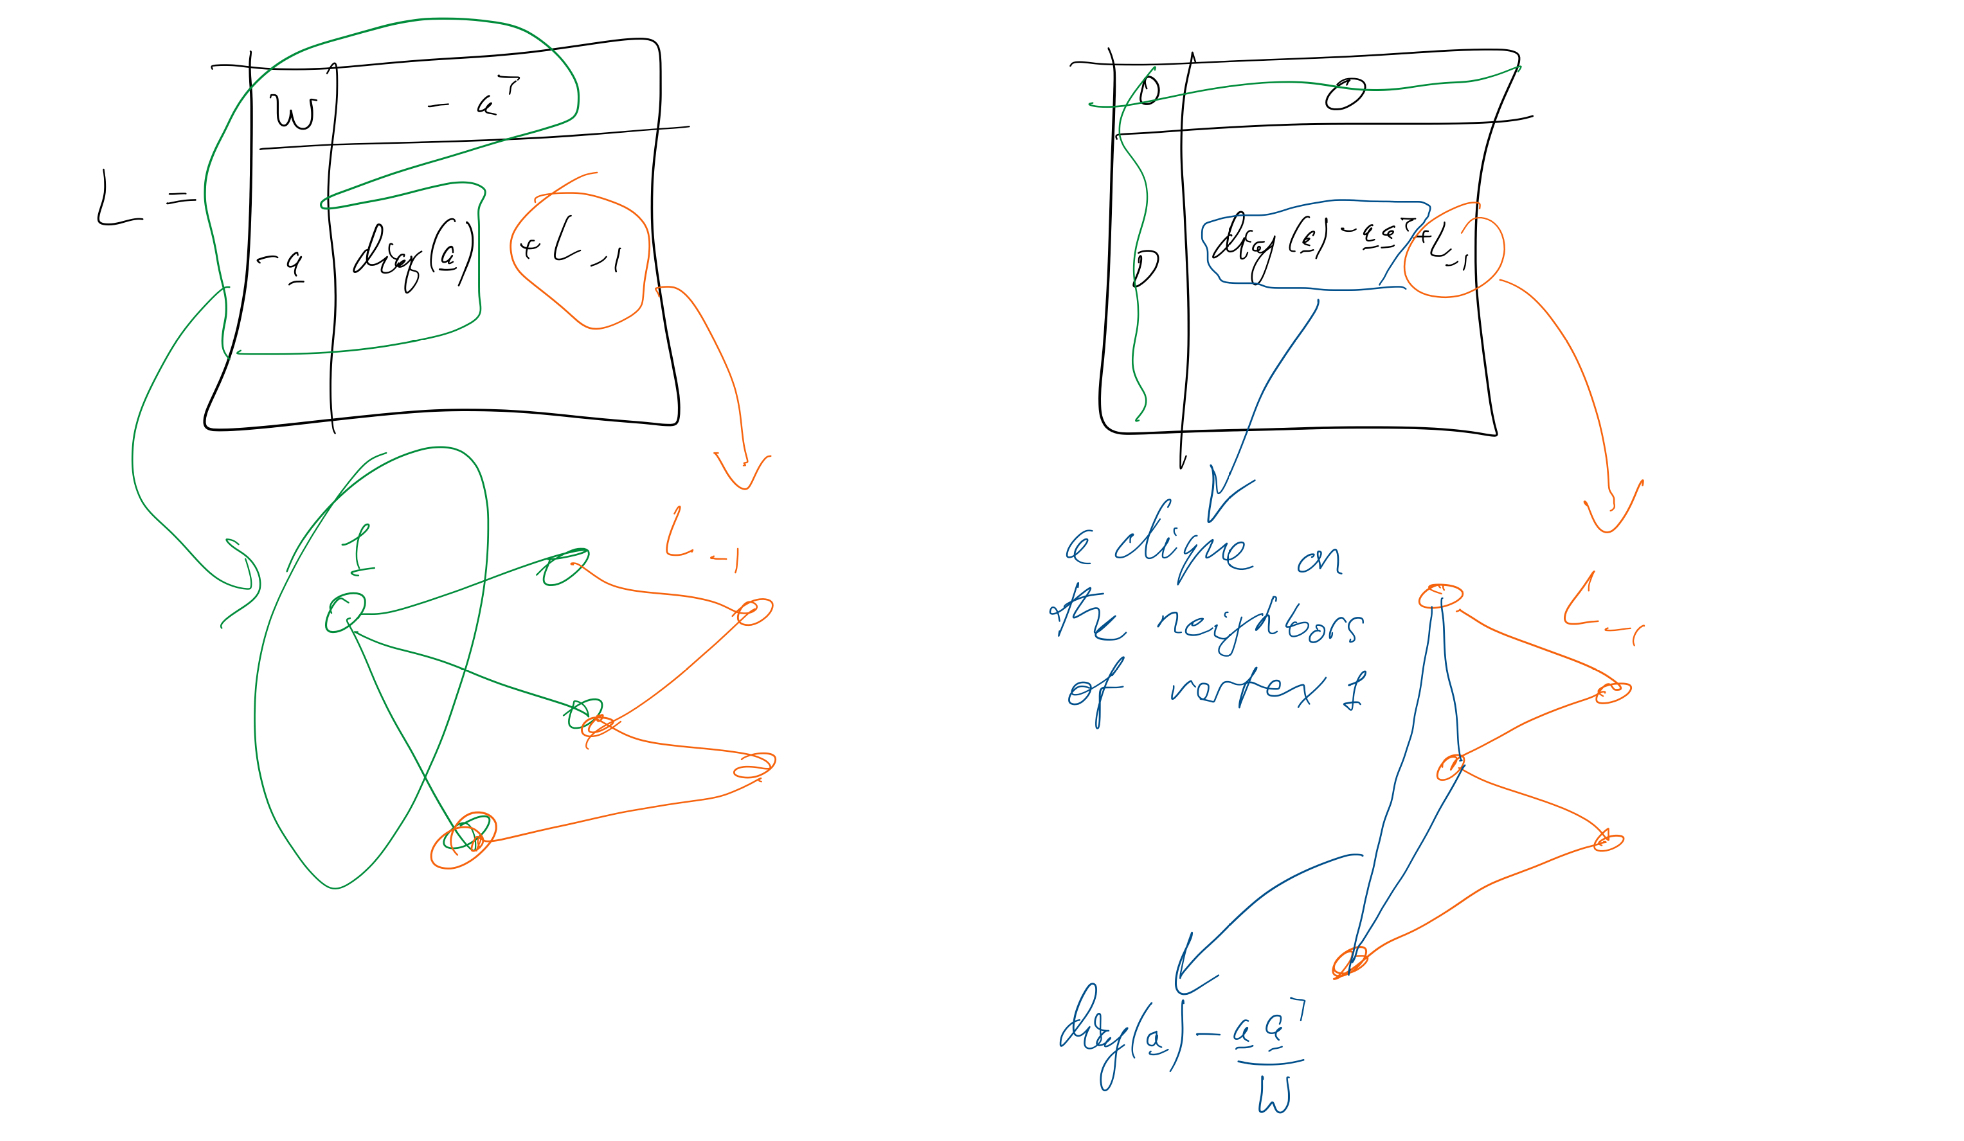
\includegraphics[width=1
  \textwidth]{fig/lecture7_schur-clique.jpeg}
% \caption{Plotting $\exp(z)$ compared to $1+z+z^2$.}
\label{fig:schurclique}
\end{figure}

\section{An Additive View of Gaussian Elimination}

\paragraph{Cholesky decomposition basics.}  Again we consider a graph Laplacian $\LL
\in \R^{n \times n}$ of a conected graph $G = (V,E,\ww)$, where as usual
$\abs{V} = n$ and $\abs{E} = m$.

In this Section, we'll study how to decompose a graph Laplacian as $\LL = \matlow \matlow^\trp$, where $\matlow \in \R^{n \times n}$
is a lower triangular matrix, i.e.
$\matlow(i,j) = 0$ for $i < j$.
Such a factorization is called a Cholesky
decomposition. It is essentially the result of Gaussian elimination with a slight twist
to ensure the matrices maintained at intermediate steps of the
algorithm remain symmetric.

We use $\nnz(\AA)$ to denote the number of non-zero entries of matrix $\AA$.
\begin{lemma}
Given an \emph{invertible} square lower triangular matrix $\matlow$,
we can solve the linear equation $\matlow \yy = \bb$ in time
$O(\nnz(\matlow))$.
Similarly, given an upper triangular matrix $\matup$, we can solve
linear equations $\matup \zz = \cc$ in time $O(\nnz(\matup))$.
\end{lemma}
We omit the proof, which is a straight-forward exercise.
The algorithms for solving linear equations in upper and lower
triangular matrices are known as forward and back substitution respectively.
\begin{remark}
  Strictly speaking, the lemma requires us to have access an adjacency
  list representation of $\matlow$ so that we can quickly tell where
  the non-zero entries are.
\end{remark}

Using forward and back substitution, if we have a decomposition of an
invertible matrix $\MM$ into $\MM = \matlow \matlow^\trp$, we can now
solve linear equations in $\MM$ in time $O(\nnz(\matlow))$.

\begin{remark}
 We have learned about decompositions using a lower triangular matrix, and later we
 will see an algorithm for computing these.
 In fact, we can have more flexibility than that. From an algorithmic perspective, it is
 sufficient that there exists a permutation matrix $\PP$ s.t. $\PP
 \matlow \PP^{\trp}$ is lower triangular. If we know the ordering
 under which the matrix becomes lower triangular, we can perform
 substitution according to that order to solve linear equations in the
 matrix without having to explicitly apply a permutation to the matrix.
\end{remark}


\paragraph{Dealing with pseudoinverses.} But how can we solve a linear equation in $\LL = \matlow
\matlow^\trp$, where $\LL$ is not invertible? For graph
Laplacians we have a simple characterization the kernel, and because
of this, dealing with the lack of invertibility turns out
to be fairly easy.

We can use the following lemma which you will prove in an exercise
next week.
\begin{lemma}
  Consider a real symmetric matrix $\MM = \XX \YY \XX^\trp$, where
  $\XX$ is real and invertible and
  $\YY$ is real symmetric.
  Let $\proj_{\MM}$ denote the orthogonal projection to the image
  of $\MM$.
  Then $\MM^{\pinv} = \proj_{\MM} (\XX^\trp)^{-1}\YY^{\pinv} \XX^{-1}\proj_{\MM}$.
\end{lemma}

The factorizations $\LL = \matlow \matlow^\trp$ that we produce will
have the property that all diagonal entries of $\matlow$ are strictly
non-zero, except that $\matlow(n,n) = 0$.
From let us $\matlowhat$ as the matrix whose entries
agree with $\matlow$, except that $\matlowhat(n,n) = 1$.
Let $\calDD$ be the diagonal matrix with $\calDD(i,i) = 1$ for $i < n$
and $\calDD(n,n) = 0$.
Then $\matlow \matlow^{\trp} = \matlowhat\calDD
\matlowhat^{\trp}$, and $\matlowhat$ is invertible, and $\calDD^{\pinv} = \calDD$.
Finally, $\proj_{\LL} = \II - \frac{1}{n}\vecone\vecone^{\trp}$,
because this matrix is acts like identity on vectors orthogonal to
$\vecone$ and ensures $\proj_{\LL} \vecone = \veczero$,
and this matrix can be applied to a vector in $O(n)$ time.
Thus $\LL^{\pinv}  = \proj_{\LL}(\matlowhat^\trp)^{-1}\calDD
\matlowhat^{-1}\proj_{\LL}$, and this matrix can be applied in time $O(\nnz(\matlow))$.

\paragraph{An additive view of Gaussian Elimination.}
The following theorem describes Gaussian Elimination / Cholesky
decompostion of a graph Laplacian.
\begin{theorem}[Cholesky Decomposition on graph Laplacians]
 Let $\LL
 \in \R^{n \times n}$ be a graph Laplacian of a connected
 graph $G = (V,E,\ww)$, where
$\abs{V} = n$.
 Using Gaussian Elimination, we can compute in $O(n^3)$ time a
 factorization $\LL = \matlow\matlow^{\trp}$ where $\matlow$ is lower
 triangular, and has positive diagonal entries except $\matlow(n,n) = 0$.
\end{theorem}
\begin{proof}
  Let $\LL^{(0)} = \LL$.
We will use $\AA(:,i)$ to denote the the $i$th column of a matrix $\AA$.
Now, for $i = 1$ to $i = n-1$ we define
\[
  \ll_i = \frac{1}{\sqrt{\LL^{(i-1)}(i,i)}} \LL^{(i-1)}(:,i)
  \text{ and }
   \LL^{(i)}  = \LL^{(i-1)} - \ll_i \ll_i^{\trp}
 \]
 Finally, we let $\ll_n = \veczero_{n \times 1}$.
 We will show later that
 \begin{equation}
   \label{eq:matlowlastentry}
   \LL^{(n-1)} = \matzero_{n \times n}.
 \end{equation}
 It follows that $\LL = \sum_{i} \ll_i \ll_i^{\trp}$, provided this
 procedure is well-defined, i.e. $\LL^{(i-1)}(i,i) \neq 0$ for all $i
< n$. We will sketch a proof of this later, while also establishing
several other properties of the procedure.

Given a matrix $\AA \in \R^{n \times n}$ and $U \subseteq [n]$, we will use $\AA(U, U)$ to
denote the principal submatrix of $\AA$ obtained by restricting to the
rows and columns with index in $U$, i.e. all entries $\AA(i,j)$ where
$i,j \in U$.
\begin{claim}
  \label{clm:schurconnected}
  Fix some $i < n$.
  Let $U = \setof{i+1,\ldots,n}$.
  Then $\LL^{(i)}(i,j) = 0$ if $i \not\in U$ or $j \not\in U$.
  And $\LL^{(i)}(U, U)$ is a graph Laplacian of a connected graph on
  the vertex set $U$.
\end{claim}
From this claim, it follows that $\LL^{(i-1)}(i,i) \neq 0$ for $i<n-1$,
since a connected graph Laplacian on a graph with $\abs{U} > 1$
vertices cannot have a zero on the diagonal, and it follows that
$\LL^{(n-1)}(i,i) = 0$, because the only graph we allow on one vertex
is the empty graph. This shows Equation~\eqref{eq:matlowlastentry} holds.
\end{proof}

\begin{proof}[Sketch of proof of Claim~\ref{clm:schurconnected}]
  % We now sketch a proof of Claim~\ref{clm:schurconnected}.
We will focus on the first elimination, as the remaining are similar.
Adopting the same notation as in Equation~\eqref{eq:lapuniformlayout},
we write
 \[
\LL^{(0)} = \LL  =
\left(
\begin{array}{ccc}
W & -\aa^\trp \\
-\aa& \diag(\aa) + \LL_{-1}
\end{array} \right)
\]
and, noting that
\[
  \ll_1 \ll_1^{\trp} =
  \begin{pmatrix}
   W & -\aa^\trp \\
-\aa & \frac{1}{W} \aa \aa^{\trp}
\end{pmatrix}
\]
we see that
\[
  \LL^{(1)}  = \LL^{(0)} - \ll_1 \ll_1^{\trp} =
  \begin{pmatrix}
   0 & \veczero \\
\veczero & \diag(\aa) - \frac{1}{W} \aa \aa^{\trp}  + \LL_{-1}
\end{pmatrix}
.
\]
Thus the first row and column of $\LL^{(1)}$ are zero claimed.
It also follows by Claim~\ref{clm:optimgaussclosed} that
$\LL^{(1)}(\setof{2,\ldots,n}, \setof{2,\ldots,n})$ is the
Laplacian of a connected graph.
This proves Claim~\ref{clm:schurconnected} for the case $i = 1$.
An induction following the same pattern can be used to prove the claim
for all $i < n$.
\end{proof}





%%% Local Variables:
%%% mode: latex
%%% TeX-master: "main"
%%% TeX-engine: luatex
%%% End:





% \section{Gaussian Elimination Recap and Structure Claim}

% %Last time, we studied a convex function minimization problem, and saw
% %how solve it by coordinatewise minimizaiton, which I claimed is really
% %Gaussian elimination in disguise.
% %Let's recap part of what we saw.

% Consider a Laplacian $\LL$ of a connected graph $G = (V,E,\ww)$, where
% $\ww \in \R^E$ is a vector of positive edge weights.
% Let $\WW \in \R^{E \times E}$ be the diagonal matrix with the edge
% weights on the diagonal, i.e. $\WW = \diag(\ww)$ and
% $\LL = \BB\WW\BB^\trp$.
% Let $\dd \in \R^V$ be a demand vector s.t. $ \dd \perp \vecone$.

% We defined an energy
% \[
%   \energy(\xx) =
% -\dd^\trp\xx +
%   \frac{1}{2}\xx^\trp\LL\xx
% \]

% Note that this function is convex and is minimized at $\xx$ s.t. $\LL
% \xx = \dd$.

% To understand how to minimize over the first variable, we
% introduce some notation for the first row and column of the Laplacian:
% \begin{equation}
%   \label{eq:lapuniformlayout}
%   \LL =
% \left(
% \begin{array}{ccc}
% W & -\aa^\trp \\
% -\aa& \diag(\aa) + \LL_{-1}
% \end{array} \right)
% \end{equation}
% Note that $W$ is the weighted degree of vertex 1, and that
% \begin{equation}
% \begin{pmatrix}
% W & -\aa^\trp \\
% -\aa& \diag(\aa)
% \end{pmatrix}
% \end{equation}
% is the Laplacian of the subgraph of $G$ containing only the edges incident on
% vertex 1, while $\LL_{-1}$ is the Laplacian of the subgraph of $G$
% containing all edges \emph{not} incident on vertex 1.

% Let us also write $\dd =
% \begin{pmatrix}
%   b \\ \cc
% \end{pmatrix}$ where $y \in \R$ and $\cc \in \R^{V \setminus
%   \setof{1}}$.

% Now,
% \begin{align*}
%   \energy(\xx)
%   &=
%   -\dd^\trp\xx +
%   \frac{1}{2}\xx^\trp\LL\xx
%   =
%   -\begin{pmatrix}
%   b \\ \cc
% \end{pmatrix}^\trp \begin{pmatrix}
%   y \\ \zz
% \end{pmatrix}
% +
%   \frac{1}{2}\begin{pmatrix}
%   y \\ \zz
% \end{pmatrix}^\trp
% \left(
% \begin{array}{ccc}
% W & -\aa^\trp \\
% -\aa& \diag(\aa) + \LL_{-1}
% \end{array} \right)
% \begin{pmatrix}
%   y \\ \zz
% \end{pmatrix}
% \end{align*}
% Now, to minimize over $y$, we set $\frac{\partial  }{\partial  y}
% \energy(\xx) = 0$ and get
% \[
%     - b
%     +
%     y W - \aa^\trp \zz
%     = 0
%    .
%   \]
%   Solving for $y$, we get that the minimizing $y$ is
% \begin{equation}
% \label{eq:laponevarmin}
% y = \frac{1}{W}(b + \aa^\trp \zz).
% \end{equation}
% By substituting in this value of $y$, we found
% \begin{align*}
%   \min_{y}
%   \energy
%   \begin{pmatrix}
%   y \\ \zz
% \end{pmatrix}
%   &=
%   -\left(\cc +  b \frac{1}{W}\aa \right)^\trp\zz
%     -
%     \frac{b^2}{2W}
%     +
%     \frac{1}{2}
%     \zz^\trp\SS \zz
%     .
% \end{align*}
% where
%  $\SS = \diag(\aa) -
%  \frac{1}{W}\aa\aa^\trp +\LL_{-1}$.
%  We let $\dd' = \cc +  b \frac{1}{W}\aa$, and $\energy'(\zz) =   -\dd^\trp\zz
% +
%     \frac{1}{2}
%     \zz^\trp\SS \zz
%     $, and noted that
% \begin{align*}
%   \argmin_{\zz} \min_{y}
%   \energy
%   \begin{pmatrix}
%   y \\ \zz
% \end{pmatrix}
%   =
% \argmin_{\zz}
%     \energy'(\zz),
% \end{align*}
%  and we ended the lecture by stating with the following claim.
%  \begin{claim}
% \label{clm:optimgaussclosed}
% \noindent
%   \begin{enumerate}
%   \item $ \dd' \perp \vecone$ when $\dd \perp \vecone$.
%   \item $\SS = \diag(\aa) - \frac{1}{W}\aa\aa^\trp +\LL_{-1} $ is a
%     Laplacian of a connected graph on the vertex set $V\setminus\setof{1}$.
%   \end{enumerate}
% \end{claim}
% Now we're ready to prove it.